\section{StrongLoop LoopBack}
\label{sec:TCH_loopback}

In this section there will be an overview about LoopBack.

Built on top of the open source LoopBack framework, the StrongLoop API Platform is the first end-to-end platform for the full API lifecycle that allows you to visually develop REST APIs in Node and get them connected to new and legacy data. In addition, the API Platform features built-in mBaaS features like push and offline sync, plus graphical tools with DevOps features for clustering, profiling and monitoring Node apps.

LoopBack generates model API from the models schemas, to let CRUD operations on models.

LoopBack models automaticaly have a standard set of HTTP endpoints that provide REST APIs for create, read, update, and delete (CRUD) operations on model data:
\begin{itemize}
\item POST /Model — Create a new instance of the model and persist it into the data source.
\item GET /Model — Find all instances of the model matched by filter from the data source.
\item PUT /Model — Update an existing model instance or insert a new one into the data source.
\item PUT /Model/{id} — Update attributes for a model instance and persist it into the data source.
\item GET /Model/{id} — Find a model instance by id from the data source.
\item DELETE /Model/{id} — Delete a model instance by id from the data source.
\item GET /Model/count — Count instances of the model matched by where from the data source.
\item GET /Model/findOne Find first instance of the model matched by filter from the data source.
\item POST /Model/update — Update instances of the model matched by where from that data source.
\end{itemize}


\begin {figure}[h]
\graphicspath{{images/chapter_TCH/}}
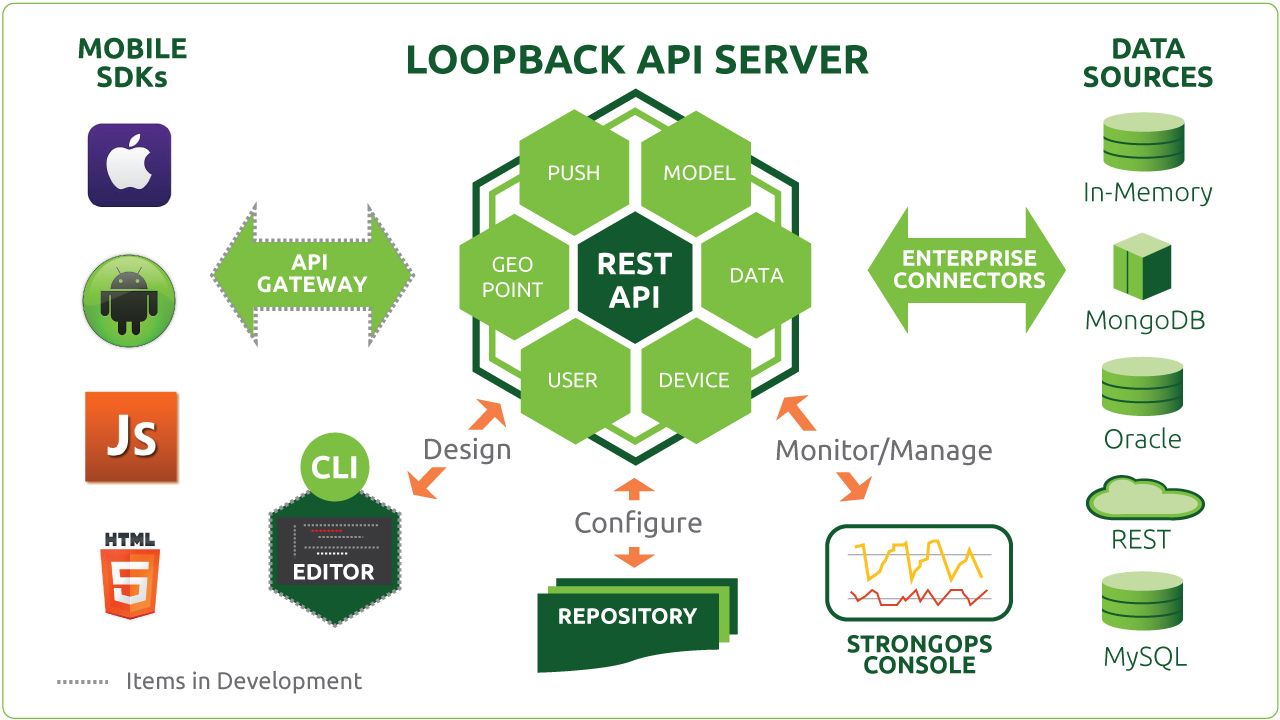
\includegraphics[width=\textwidth]{loopback_1}
\caption{LoopBack Architecture}
\end {figure}



A LoopBack model represents data in backend systems such as databases, and by default has both Node and REST APIs.  Additionally, developer can add functionality such as validation rules and business logic to models.
Every LoopBack application has a set of predefined built-in models such as User, Role, and Application.  Developer can extend built-in models to suit your application's needs.

The model JSON file defines models, relations between models, and access to models. 

\begin{lstlisting}[language=javascript]
{
  "name": "ModelName",  // See Top-level properties below
  "description": "A Customer model representing our customers.",
  "base": "User",
  "idInjection": false,
  "strict": true,
  "options": { ... }, // See Options below
  "properties": { ... }, // See Properties below
  "validations": [...],  // See Validations below
  "relations": {...},  // See Relations below
  "acls": [...],  // See ACLs below
  "scopes": {...},  // See Scopes below
  "http": {"path": "/foo/mypath"}
}
\end{lstlisting}

\subsection{Top-level Properties}

\textbf{Name}

Name of the model.

\textbf{Description}

Optional description of the model.

\textbf{Base}

Name of another model that this model extends. The model will ``inheri'' properties and methods of the base model.

\textbf{IdInjection}

Whether to automatically add an id property to the model:
\begin{itemize}
\item true id property is added to the model automatically. This is the default.
\item false id property is not added to the model.
\end{itemize}

\textbf{Strict}

Specifies whether the model accepts only predefined properties or not. One of:
\begin{itemize}
\item true Only properties defined in the model are accepted. Use if you want to ensure the model accepts only predefined properties.
\item false The model is an open model and accepts all properties, including ones not predefined in the model. This mode is useful to store free-form JSON data to a schema-less database such as MongoDB.
\item validate The unknown properties will be reported as validation errors.
\item throw Throws an exception if properties not defined for the model are used in an operation.
\item Undefined Defaults to false unless the data source is backed by a relational database such as Oracle or MySQL.
\end{itemize}

\textbf{Options}

JSON object that specifies model options.

\textbf{Properties}

JSON object that specifies the properties in the model.

\textbf{Relations}

Object containing relation names and relation definitions.

\textbf{Acls}

Set of ACL specifications that describes access control for the model.

The API can be extended: the developer can add remote functions to mod- els or add hooks to existing API to add custom behavior before and/or after the API handler (to pre-process the re-quest and/or post-process the response). The resulting API is RESTful, cookie free, signed by authentication token. By default, applications have a built-in model that represents a user, with properties username, email and password and role for authentication and authorization. Loopback also introduces an indirection layer that allows to choose from almost all particular DBMS to be used.
